\documentclass[usenames,dvipsnames]{beamer}
\usetheme[deutsch]{KIT}

\usepackage[utf8]{inputenc}
\usepackage[T1]{fontenc}
\usepackage{babel}
\usepackage{tikz,calc,ifthen}
\usetikzlibrary{shapes.geometric}
\usetikzlibrary{positioning}
\usepackage{mathtools}
\usepackage[normalem]{ulem}
\usepackage{graphicx}
\usepackage{minted}
\usepackage{booktabs}
\usetikzlibrary{positioning,calc,arrows,shapes}
\tikzset{
  every node/.style={transform shape},
  auto,
  block/.style={align=center,rectangle,draw,minimum height=20pt,minimum width=30pt},
  >=triangle 60,
  alt/.code args={<#1>#2#3}{%
      \alt<#1>{\pgfkeysalso{#2}}{\pgfkeysalso{#3}}
  },
  beameralert/.style={alt=<#1>{color=green!80!black}{}},
  mythick/.style={line width=1.4pt}
}

\newcommand*{\maxwidthofm}[2]{\maxof{\widthof{$#1$}}{\widthof{$#2$}}}
\newcommand<>*{\robustaltm}[2]{
  \alt#3
  {\mathmakebox[\maxwidthofm{#1}{#2}]{#1}\vphantom{#1#2}}
    {\mathmakebox[\maxwidthofm{#1}{#2}]{#2}\vphantom{#1#2}}
}

\newcommand<>*{\nodealert}[1]{\only#2{\draw[overlay,mythick,color=green!80!black] (#1.north west) rectangle (#1.south east)}}

\title{Schleifenausrollen mit nicht konstanten Grenzen in FIRM}
\author{Adrian E. Lehmann}
\subtitle{\insertauthor}
\institute[IPD]{Lehrstuhl Programmierparadigmen, IPD Snelting}
\date{04.10.2019}
\KITtitleimage{Cover.jpeg}

\begin{document}

\begin{frame}
  \maketitle
\end{frame}

\begin{frame}{Ausrollen}
  \begin{center}
    \inputminted{c}{code_snippets/01-00-const-bound.c}
  \end{center}
\end{frame}

\begin{frame}{Ausrollen}
  \begin{center}
    \inputminted{c}{code_snippets/01-01-const-bound-unrolled.c}
  \end{center}
\end{frame}

\begin{frame}{Ausrollen: Nicht konstante Grenze}
  \begin{center}
    \inputminted{c}{code_snippets/02-00-non-const-bound.c}
    \only<2>{
      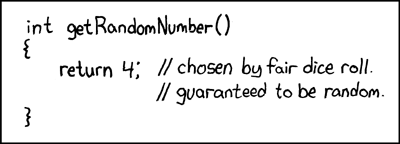
\includegraphics[width=0.5\textwidth]{fig/xkcd_random_number.png}\\
      \texttt{https://xkcd.com/221/}
    }
    \only<3>{\texttt{fairDiceRoll()} $\in \lbrack 1, 6 \rbrack$ (random)}
  \end{center}
\end{frame}

\begin{frame}{Ausrollen: Nicht konstante Grenze}
  \begin{center}
    \inputminted{c}{code_snippets/02-01-non-const-bound-unrolled.c}
  \end{center}
  $\hookrightarrow$ \texttt{length} $\in \{\only<2->{\color{red}} 1, \only<2>{\normalcolor} 2, \only<2-3>{\normalcolor} 3, \only<4->{\normalcolor} 4,\only<5-6>{\color{red}} 5, \only<5>{\normalcolor} 6\normalcolor \}$
\end{frame}

\begin{frame}{Ausrollen: Nicht konstante Grenze}
  \begin{center}
    \inputminted{c}{code_snippets/03-00-non-const-bound-unrolled-less.c}
  \end{center}
  $\hookrightarrow$ \texttt{length} $\in \{\only<2->{\color{orange}} 1, \only<2>{\normalcolor} 2, \only<2-3>{\normalcolor} 3, \only<4->{\normalcolor} 4,\only<5-6>{\color{orange}} 5, \only<5>{\normalcolor} 6\normalcolor \}$
\end{frame}

\begin{frame}{Nicht konstante Grenze: Naiver Ansatz}
  \begin{center}
    \inputminted{c}{code_snippets/04-00-non-const-bound-loop-fixup.c}
  \end{center}
  $\hookrightarrow$ \texttt{length} $\in \{\only<2>{\color{green}} 1, 2, 3, \normalcolor 4,\only<2>{\color{green}} 5, 6\normalcolor \}$
\end{frame}

\begin{frame}{Problem}
  \begin{center}
    \inputminted{c}{code_snippets/04-02-non-const-bound-loop-fixup-unsigned.c}
  \end{center}
  $\hookrightarrow$ \texttt{length} $\in \{\only<3>{\color{red}} 1, 2,\only<2->{\color{green}} 3, \normalcolor 4,\only<2->{\color{green}} 5, 6\normalcolor \}$
\end{frame}

\begin{frame}{Lösung}
  \begin{center}
    \inputminted{c}{code_snippets/04-03-non-const-bound-loop-fixup-unsigned-fixed.c}
  \end{center}
  $\hookrightarrow$ \texttt{length} $\in \{\only<3>{\color{green}} 1, 2,\only<2->{\color{green}} 3, \normalcolor 4,\only<2->{\color{green}} 5, 6\normalcolor \}$
\end{frame}

\begin{frame}{Nicht konstante Grenze: Duff's Device}
  \begin{center}
    \inputminted{c}{code_snippets/04-01-non-const-bound-duff-fixup.c}
  \end{center}
  $\hookrightarrow$ \texttt{length} $\in \{\only<2>{\color{green}} 1, 2, 3, \normalcolor 4,\only<2>{\color{green}} 5, 6\normalcolor \}$
\end{frame}

\begin{frame}{Nicht konstante Grenze: Allgemeine Schleife}
  \begin{center}
    \inputminted{c}{code_snippets/10-00-general-loop.c}
  \end{center}
  \begin{itemize}
    \item $f$ Ausrollfaktor
    \item $N$ Scheilfen invariant
    \item $c \in \lbrack \frac{t_{min}}{f + 1}, \frac{t_{max}}{f + 1} \rbrack$
    \item $cmp \in \{<,\leq,>,\geq\}$
  \end{itemize}
\end{frame}

\begin{frame}{$c$ ist Streckung}
  \begin{center}
    \only<1> {
      \inputminted{c}{code_snippets/10-05-stretch-01.c}
    }
    \only<2>{
      \inputminted{c}{code_snippets/10-06-stretch-02.c}
    }
  \end{center}
\end{frame}

\begin{frame}{Allgemeine Schleife in FIRM}
  \begin{center}
    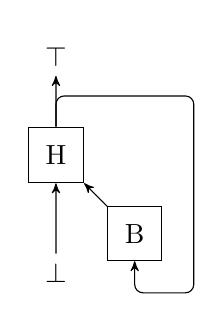
\begin{tikzpicture}[->,>=stealth',square/.style={regular polygon,regular polygon sides=4}]
    \node at (0, 0.25) (pre) {$\top$};
    \node at (0, -1) [square, draw] (H) {H};
    \node at (1, -2) [square, draw] (B) {B};
    \node at (0, -2.5) (post) {$\bot$};
    \node at (1.5, 0.5) (poi0) {};
    \node at (1.5, -2.5) (poi1) {};
    \path[every node/.style={font=\sffamily\small}]
    (H) edge node [right] {} (pre)
    (post) edge node [right] {} (H)
    (B) edge node [right] {} (H);

    \draw[rounded corners=3pt, <-] (B.south) -- (1,-2.75) -- (1.75,-2.75) -- (1.75,-0.25) -- (0, -0.25) -- (H.north);

\end{tikzpicture}
  \end{center}
\end{frame}

\begin{frame}{Allgmeiner Loop fixup}
  \begin{center}
    \inputminted{c}{code_snippets/13-00-general-loop-fixup-preheader.c}
  \end{center}
  $c \in \lbrack \frac{t_{min}}{f + 1}, \frac{t_{max}}{f + 1} \rbrack$\\
\end{frame}

\begin{frame}{Allgemeiner Loop fixup in FIRM}
  \begin{center}
    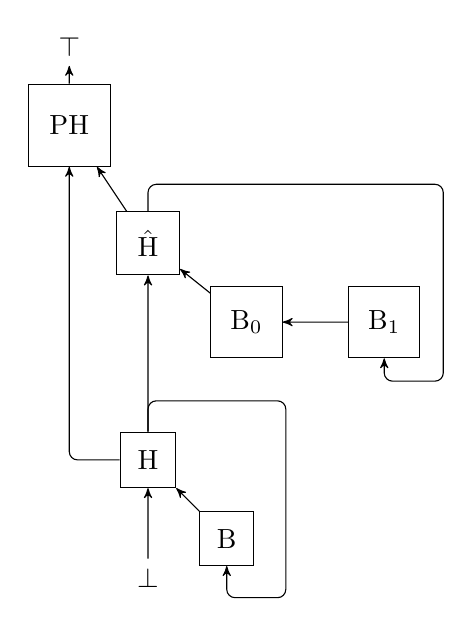
\begin{tikzpicture}[->,>=stealth',square/.style={regular polygon,regular polygon sides=4}]
    \node at (-1, 1.5) (pre) {$\top$};
    \node at (-1, 0.5) [square, draw] (PH) {PH};
    \node at (0, -1) [square, draw] (H) {$\hat{\text{H}}$};
    \node at (1.25, -2) [square, draw] (B) {B\textsubscript{0}};
    \node at (3, -2) [square, draw] (BDup) {B\textsubscript{1}};
    \node at (0, -3.75) [square, draw] (H1) {H};
    \node at (1, -4.75) [square, draw] (B1) {B};
    \node at (0, -5.25) (post) {$\bot$};
    \path[every node/.style={font=\sffamily\small}]
    (PH) edge node [right] {} (pre)
    (H) edge node [right] {} (PH)

    (H1) edge node [right] {} (H)
    (post) edge node [right] {} (H1)

    (B) edge node [right] {} (H)
    (BDup) edge node [right] {} (B)
    (B1) edge node [right] {} (H1);


    \draw[rounded corners=3pt, <-] (BDup.south) -- (3,-2.75) -- (3.75,-2.75) -- (3.75,-0.25) -- (0, -0.25) -- (H.north);
    \draw[rounded corners=3pt, <-] (B1.south) -- (1,-5.5) -- (1.75,-5.5) -- (1.75,-3) -- (0, -3) -- (H1.north);
    \draw[rounded corners=3pt, ->] (H1.west) -- (-1,-3.75) -- (PH.south);
\end{tikzpicture}
  \end{center}
\end{frame}

\begin{frame}{Allgemeiner Duff's Device fixup}
  \begin{center}
    \inputminted{c}{code_snippets/14-00-general-duff-fixup.c}
  \end{center}
  \begin{itemize}
    \item $c \in \lbrack \frac{t_{min}}{f + 1}, \frac{t_{max}}{f + 1} \rbrack$
  \end{itemize}
\end{frame}

\begin{frame}{Allgemeiner Duff's Device fixup in FIRM}
  \begin{center}
    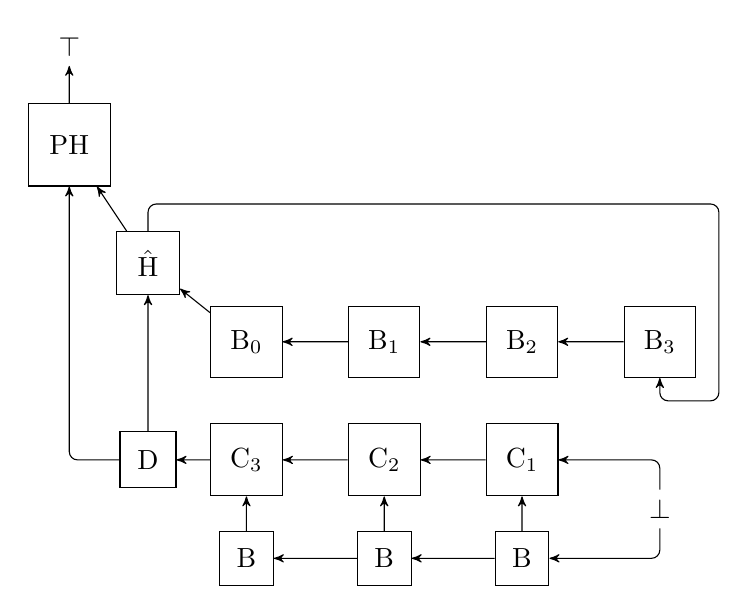
\begin{tikzpicture}[->,>=stealth',square/.style={regular polygon,regular polygon sides=4}]
    \node at (-1, 1.75) (pre) {$\top$};
    \node at (-1, 0.5) [square, draw] (PH) {PH};
    \node at (0, -1) [square, draw] (H) {$\hat{\text{H}}$};
    \node at (1.25, -2) [square, draw] (B) {B\textsubscript{0}};
    \node at (3, -2) [square, draw] (BDup1) {B\textsubscript{1}};
    \node at (4.75, -2) [square, draw] (BDup2) {B\textsubscript{2}};
    \node at (6.5, -2) [square, draw] (BDup3) {B\textsubscript{3}};
    \node at (0, -3.5) [square, draw] (H1) {D};
    \node at (1.25, -3.5) [square, draw] (C0) {C\textsubscript{3}};
    \node at (3, -3.5) [square, draw] (C1) {C\textsubscript{2}};
    \node at (4.75, -3.5) [square, draw] (C2) {C\textsubscript{1}};

    \node at (1.25, -4.75) [square, draw] (B0) {B};
    \node at (3, -4.75) [square, draw] (B1) {B};
    \node at (4.75, -4.75) [square, draw] (B2) {B};
    \node at (6.5, -4.125) (post) {$\bot$};
    \path[every node/.style={font=\sffamily\small}]
    (PH) edge node [right] {} (pre)
    (H) edge node [right] {} (PH)

    (H1) edge node [right] {} (H)

    (B) edge node [right] {} (H)
    (BDup1) edge node [right] {} (B)
    (BDup2) edge node [right] {} (BDup1)
    (BDup3) edge node [right] {} (BDup2)


    (C1) edge node [right] {} (C0)
    (C2) edge node [right] {} (C1)

    (B1) edge node [right] {} (B0)
    (B2) edge node [right] {} (B1)

    (B0) edge node [right] {} (C0)
    (B1) edge node [right] {} (C1)
    (B2) edge node [right] {} (C2);


    \draw[rounded corners=3pt, ->] (C0.west) -- (H1.east);
    \draw[rounded corners=3pt, <-] (BDup3.south) -- (6.5,-2.75) -- (7.25,-2.75) -- (7.25,-0.25) -- (0, -0.25) -- (H.north);
    \draw[rounded corners=3pt, ->] (post.south) -- (6.5, -4.75) -- (B2.east);
    \draw[rounded corners=3pt, ->] (post.north) -- (6.5, -3.5) -- (C2.east);
    \draw[rounded corners=3pt, ->] (H1.west) -- (-1,-3.5) -- (PH.south);
\end{tikzpicture}
  \end{center}
\end{frame}

\begin{frame}{Benchmarks}
  %\begin{tabular}{l|rrrrrr}
   % Maximum size & 32 & 64  & 128 & 256 & 512 & 1024\\
    %\toprule
    %\textbf{Loop fixup} & 99.44\% & 99.47\% & 100.00\% & 100.32\% & 99.99\% & 100.24\%\\
    %\textbf{Duff's Device fixup} & 99.79\% & 100.12\% & 100.27\% & 99.53\% & 99.47\% & 100.35\%\\
  %\end{tabular}
  \begin{center}
    \begin{tabular}{l|rr}
      Maximum size & Loop fixup & Duff's Device fixup\\
      \toprule
      32 & 99.44\% & 99.79\% \\
      64 & 99.47\% & 100.12\% \\
      128 & 100.00\% & 100.27\% \\
      256 & 100.32\% & 99.53\% \\
      512 & 99.99\% & 99.47\% \\
      1024 & 100.24\% & 100.35\%\\
    \end{tabular}
    \vspace{12pt}
    \\
    Vergleich zur Referenz ohne Schleifenausrollen
    \vspace{12pt}

    Ausrei\ss{}er: \texttt{h264ref}
  \end{center}
\end{frame}

\begin{frame}{Evalulation \& Überblick}
  \begin{itemize}
    \item LCSSA hilfreich
    \item BA Aebi, gute Grundlage\pause
    \item Doppelt so viele Schleifen ausgerollt
    \item Kein Performancegewinn\pause
    \item >2.5 KLOC
    \item ca. 5 Beweise nötig
  \end{itemize}
\end{frame}

\begin{frame}{Zusammenfassung}
  \begin{itemize}
    \item Nicht konstante Grenze ausrollbar
    \item Grenze invariant, Inkrement konstant
    \item Spekulativ ausrollen
    \item Weniger oder gleich viele Ausführungen
    \item Fixup code entweder Loop oder Duff's Device
    \item Preheader für Overflows
  \end{itemize}
\end{frame}
\end{document}
